\documentclass[11pt,a4paper]{article}

\usepackage{../../templates/style}

\begin{document}

\begin{problem}{Road Cut}{standard input}{standard output}{1 second}{64 megabytes}

คณะกรรมการผู้บริหารเมืองแห่งหนึ่งต้องการทำการตัดถนนผ่านพื้นที่ใจกลางเมือง โดยความต้องการของเมืองคือการตัดถนนเป็นเส้นตรงผ่านเมืองเป็นเส้นตรงทางทิศทางใดก็ได้ ระหว่างการตัดถนนผ่านทางด้านทิศตะวันตกไปยังด้านทิศตะวันออก (ซ้ายไปขวา) หรือทางด้านทิศเหนือไปยังด้านทิศใต้ (บนลงล่าง) ซึ่งพื้นที่ดังกล่าวมีมูลค่าของพื้นที่ในแต่ละส่วนไม่เท่ากัน  นอกเหนือจากนั้นเมื่อตัดถนนแล้วจะทำให้พื้นที่ที่อยู่ติดถนนมีมูลค่าสูงขึ้น เพื่อให้การตัดถนนทำให้เกิดความเสียหายน้อยที่สุดและเพื่อประโยชน์ของเมืองโดยรวม การตัดถนนจึงควรตัดผ่านพื้นที่ที่มีมูลค่าต่ำที่สุดและยังทำให้มูลค่าพื้นที่โดยรวมของเมืองมีมูลค่าเพิ่มขึ้นสูงสุดอีกด้วย

\begin{figure}[h]
\centering
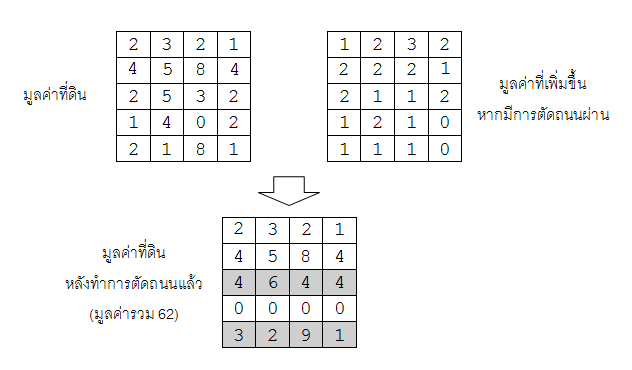
\includegraphics[width=0.9\textwidth]{../latex/img/1044/1044-1.png}
\caption{รูปตัวอย่างการสร้างถนน เมื่อสร้างถนนจากทิศตะวันตกไปยังทิศตะวันออก ในแถวที่ $4$}
\end{figure}

\bigskip
\underline{\textbf{โจทย์}}  จงเขียนโปรแกรมเพื่ออ่านข้อมูลนำเข้าของมูลค่าพื้นที่ย่อยภายในเมือง และการเปลี่ยนแปลงมูลค่าของพื้นที่ย่อยเมื่อมีการตัดถนนผ่าน ทั้งนี้กำหนดให้พื้นที่ภายในเมืองมีรูปทรงเป็นสี่เหลี่ยมผืนผ้าหรือสี่เหลี่ยมจัตุรัสเสมอ จากนั้นให้คำนวณหาเส้นทางที่ทำให้มูลค่าพื้นที่ของเมืองโดยรวมมีมูลค่าสูงที่สุดเพื่อให้คณะกรรมการนำไปพิจารณาทำการตัดถนน โดยกำหนดให้เส้นทางที่ถูกทำเป็นถนนจะมีมูลค่าพื้นที่เหลือ $0$

\InputFile

\textbf{บรรทัดแรก} รับจำนวนเต็มสองตัว $n$ $(2 < n \leq 100)$ และ $m$ $(2 < m \leq 100)$ ซึ่งเป็นขนาดของพื้นที่เมืองจากทิศเหนือไปทิศใต้ แบะจากทิศจะวันตกไปทิศตะวันออกตามลำดับ

\textbf{บรรทัดที่ $2$ ถึง $n+1$} เป็นข้อมูลของมูลค่าพื้นที่ย่อยจากเหนือลงใต้ โดยบรรทัดที่ $i+1$ จะแสดงข้อมูลของพื้นที่ย่อยในแถวที่ $i$ $(1 \leq i \leq n)$ โดยที่แต่ละบรรทัดจะมีตัวเลขจำนวนเต็มทั้งหมด $m$ ตัว, $a_1$ $a_2$ $a_3$ $...$ $a_m$ (ตัวเลขแต่ละตัวจะถูกคั่นด้วยช่องว่าง) เมื่อ $a_j$ แทนมูลค่าของที่ดินช่องที่ $j$ โดย $0 \leq a_j \leq 100$ 


\textbf{บรรทัดที่ $n+2$ ถึง $2n+1$} เป็นข้อมูลการเปลี่ยนแปลงมูลค่าของพื้นที่ย่อยเมื่อมีถนนตัดผ่าน โดยบรรทัดที่ $n+i+1$ จะแสดงข้อมูลของการเปลี่ยนแปลงมูลค่าพื้นที่ย่อยในแถวที่ $i$ $(1 \leq i \leq n)$ โดยที่แต่ละบรรทัดจะมีตัวเลขทั้งหมด $m$ ตัว, $b_1$ $b_2$ $b_3$ $...$ $b_m$ (ตัวเลขแต่ละตัวจะถูกคั่นด้วยช่องว่าง) เมื่อ $b_j$ แทนมูลค่าของที่ดินช่องที่ $j$ โดย $0 \leq b_j \leq 20$ (ซึ่งอาจจะทำให้มูลค่าของพื้นที่ย่อยมีค่าเกิน $100$ ได้)

\OutputFile

\textbf{มีบรรทัดเดียว} แสดงตัวเลข $1$ ตัวซึ่งแสดงถึงมูลค่ารวมของพื้นที่ภายในเมืองหลังจากทำการตัดถนนเรียบร้อยแล้ว

\Examples

\begin{example}
\exmp{5 4
2 3 2 1
4 5 8 4
2 5 3 2
1 4 0 2
2 1 8 1
1 2 3 2
2 2 2 1
2 1 1 2
1 2 1 0
1 1 1 0}{62}%
\end{example}


\Source

การแข่งขันคณิตศาสตร์ วิทยาศาสตร์ โอลิมปิกแห่งประเทศไทย สาขาวิชาคอมพิวเตอร์ ประจำปี 2550

\end{problem}

\end{document}